\documentclass[twocolumn,11pts]{IEEEtran}
% packages to make the language spanish
\usepackage[spanish,es-lcroman,es-tabla,es-nosectiondot]{babel}
\decimalpoint% changes the coma in the numbers to period
\usepackage[utf8]{inputenc}
\usepackage[T1]{fontenc}
\usepackage{csquotes}


% Some very useful LaTeX packages include:
% (uncomment the ones you want to load)

% *** CAPTION ***
\usepackage[font=footnotesize,labelfont=bf,labelsep=period]{caption}

% *** CITATION PACKAGES ***
%
\usepackage{cite}
%
% cite.sty was written by Donald Arseneau
% V1.6 and later of IEEEtran pre-defines the format of the cite.sty package
% \cite{} output to follow that of IEEE. Loading the cite package will
% result in citation numbers being automatically sorted and properly
% "compressed/ranged". e.g., [1], [9], [2], [7], [5], [6] without using
% cite.sty will become [1], [2], [5]--[7], [9] using cite.sty. cite.sty's
% \cite will automatically add leading space, if needed. Use cite.sty's
% noadjust option (cite.sty V3.8 and later) if you want to turn this off.
% cite.sty is already installed on most LaTeX systems. Be sure and use
% version 4.0 (2003-05-27) and later if using hyperref.sty. cite.sty does
% not currently provide for hyperlinked citations.
% The latest version can be obtained at:
% http://www.ctan.org/tex-archive/macros/latex/contrib/cite/
% The documentation is contained in the cite.sty file itself.

% Bibliografia para este documento
% Se incluye embebida para poder transportarla en el mismo documento. Sin embargo,
% en sus documentos puede tener esta información en el archivo *.bib.
% Consecuentemente, no necesita el uso del paquete filecontents.
\usepackage{filecontents}
\begin{filecontents}{guia.bib}
% note el uso de las llaves {} para escapar la instrucción \LaTeX dentro del título del artículo
@ARTICLE{Downes2002,
  title = {Short Math Guide for {\LaTeX}},
  author = {Michael Downes},
  year = {2002},
  url = {ftp://ftp.ams.org/pub/tex/doc/amsmath/short-math-guide.pdf}
}
\end{filecontents}


% *** GRAPHICS RELATED PACKAGES ***
%
% \usepackage[pdftex]{graphicx}
% declare the path(s) where your graphic files are
% \graphicspath{{../pdf/}{../jpeg/}}
% and their extensions so you won't have to specify these with
% every instance of \includegraphics
% \DeclareGraphicsExtensions{.pdf,.jpeg,.png}
%
% graphicx was written by David Carlisle and Sebastian Rahtz. It is
% required if you want graphics, photos, etc. graphicx.sty is already
% installed on most LaTeX systems. The latest version and documentation can
% be obtained at: 
% http://www.ctan.org/tex-archive/macros/latex/required/graphics/
% Another good source of documentation is "Using Imported Graphics in
% LaTeX2e" by Keith Reckdahl which can be found as epslatex.ps or
% epslatex.pdf at: http://www.ctan.org/tex-archive/info/
%
% latex, and pdflatex in dvi mode, support graphics in encapsulated
% postscript (.eps) format. pdflatex in pdf mode supports graphics
% in .pdf, .jpeg, .png and .mps (metapost) formats. Users should ensure
% that all non-photo figures use a vector format (.eps, .pdf, .mps) and
% not a bitmapped formats (.jpeg, .png). IEEE frowns on bitmapped formats
% which can result in "jaggedy"/blurry rendering of lines and letters as
% well as large increases in file sizes.
%
% You can find documentation about the pdfTeX application at:
% http://www.tug.org/applications/pdftex


% *** MATH PACKAGES ***
%
%\usepackage[cmex10]{amsmath}
% A popular package from the American Mathematical Society that provides
% many useful and powerful commands for dealing with mathematics. If using
% it, be sure to load this package with the cmex10 option to ensure that
% only type 1 fonts will utilized at all point sizes. Without this option,
% it is possible that some math symbols, particularly those within
% footnotes, will be rendered in bitmap form which will result in a
% document that can not be IEEE Xplore compliant!
%
% Also, note that the amsmath package sets \interdisplaylinepenalty to 10000
% thus preventing page breaks from occurring within multiline equations. Use:
%\interdisplaylinepenalty=2500
% after loading amsmath to restore such page breaks as IEEEtran.cls normally
% does. amsmath.sty is already installed on most LaTeX systems. The latest
% version and documentation can be obtained at:
% http://www.ctan.org/tex-archive/macros/latex/required/amslatex/math/


% *** SPECIALIZED LIST PACKAGES ***
%
\usepackage{algorithm}
\usepackage{algpseudocode}
\makeatletter
\renewcommand{\ALG@name}{Algoritmo}% Algorithm -> Algoritmo
\makeatother
\captionsetup[algorithm]{font=footnotesize,labelsep=period}
% algorithmic.sty was written by Peter Williams and Rogerio Brito.
% This package provides an algorithmic environment fo describing algorithms.
% You can use the algorithmic environment in-text or within a figure
% environment to provide for a floating algorithm. Do NOT use the algorithm
% floating environment provided by algorithm.sty (by the same authors) or
% algorithm2e.sty (by Christophe Fiorio) as IEEE does not use dedicated
% algorithm float types and packages that provide these will not provide
% correct IEEE style captions. The latest version and documentation of
% algorithmic.sty can be obtained at:
% http://www.ctan.org/tex-archive/macros/latex/contrib/algorithms/
% There is also a support site at:
% http://algorithms.berlios.de/index.html
% Also of interest may be the (relatively newer and more customizable)
% algorithmicx.sty package by Szasz Janos:
% http://www.ctan.org/tex-archive/macros/latex/contrib/algorithmicx/

\usepackage{listings}
\usepackage{tikz}
\lstset{
  language=[LaTeX]TeX,
  breaklines=true,
  basicstyle=\tt\scriptsize,
  keywordstyle=\color{blue},
  identifierstyle=\color{magenta},
  commentstyle=\color{green!40!black},
  % frame 
  frame=tb,
  captionpos=t,
  xleftmargin=1em,
  numbersep=0.3em,
  numbers=left,
  framexleftmargin=1.1em,
  framexrightmargin=0pt,
  % additional letters for accents in spanish
  literate=%
    {á}{{\'{a}}}1
    {é}{{\'{e}}}1
    {í}{{\'{i}}}1
    {ó}{{\'{o}}}1
    {ú}{{\'{u}}}1
    {ñ}{{\~{n}}}1
    {Ñ}{{\~{N}}}1
}

\renewcommand{\lstlistingname}{Código}% Listing -> Código
\DeclareCaptionFormat{listing}{\rule{\dimexpr\linewidth\relax}{0.4pt}\par\vskip1pt#1#2#3}
\captionsetup[lstlisting]{format=listing,singlelinecheck=false, margin=0pt,position=bottom}

% *** ALIGNMENT PACKAGES ***
%
%\usepackage{array}
% Frank Mittelbach's and David Carlisle's array.sty patches and improves
% the standard LaTeX2e array and tabular environments to provide better
% appearance and additional user controls. As the default LaTeX2e table
% generation code is lacking to the point of almost being broken with
% respect to the quality of the end results, all users are strongly
% advised to use an enhanced (at the very least that provided by array.sty)
% set of table tools. array.sty is already installed on most systems. The
% latest version and documentation can be obtained at:
% http://www.ctan.org/tex-archive/macros/latex/required/tools/


%\usepackage{mdwmath}
%\usepackage{mdwtab}
% Also highly recommended is Mark Wooding's extremely powerful MDW tools,
% especially mdwmath.sty and mdwtab.sty which are used to format equations
% and tables, respectively. The MDWtools set is already installed on most
% LaTeX systems. The lastest version and documentation is available at:
% http://www.ctan.org/tex-archive/macros/latex/contrib/mdwtools/


% IEEEtran contains the IEEEeqnarray family of commands that can be used to
% generate multiline equations as well as matrices, tables, etc., of high
% quality.


%\usepackage{eqparbox}
% Also of notable interest is Scott Pakin's eqparbox package for creating
% (automatically sized) equal width boxes - aka "natural width parboxes".
% Available at:
% http://www.ctan.org/tex-archive/macros/latex/contrib/eqparbox/


% *** SUBFIGURE PACKAGES ***
%\usepackage[tight,footnotesize]{subfigure}
% subfigure.sty was written by Steven Douglas Cochran. This package makes it
% easy to put subfigures in your figures. e.g., "Figure 1a and 1b". For IEEE
% work, it is a good idea to load it with the tight package option to reduce
% the amount of white space around the subfigures. subfigure.sty is already
% installed on most LaTeX systems. The latest version and documentation can
% be obtained at:
% http://www.ctan.org/tex-archive/obsolete/macros/latex/contrib/subfigure/
% subfigure.sty has been superceeded by subfig.sty.


%\usepackage[caption=false]{caption}
%\usepackage[font=footnotesize]{subfig}
% subfig.sty, also written by Steven Douglas Cochran, is the modern
% replacement for subfigure.sty. However, subfig.sty requires and
% automatically loads Axel Sommerfeldt's caption.sty which will override
% IEEEtran.cls handling of captions and this will result in nonIEEE style
% figure/table captions. To prevent this problem, be sure and preload
% caption.sty with its "caption=false" package option. This is will preserve
% IEEEtran.cls handing of captions. Version 1.3 (2005/06/28) and later 
% (recommended due to many improvements over 1.2) of subfig.sty supports
% the caption=false option directly:
\usepackage[caption=false,font=footnotesize]{subfig}
%
% The latest version and documentation can be obtained at:
% http://www.ctan.org/tex-archive/macros/latex/contrib/subfig/
% The latest version and documentation of caption.sty can be obtained at:
% http://www.ctan.org/tex-archive/macros/latex/contrib/caption/


% *** FLOAT PACKAGES ***
%
%\usepackage{fixltx2e}
% fixltx2e, the successor to the earlier fix2col.sty, was written by
% Frank Mittelbach and David Carlisle. This package corrects a few problems
% in the LaTeX2e kernel, the most notable of which is that in current
% LaTeX2e releases, the ordering of single and double column floats is not
% guaranteed to be preserved. Thus, an unpatched LaTeX2e can allow a
% single column figure to be placed prior to an earlier double column
% figure. The latest version and documentation can be found at:
% http://www.ctan.org/tex-archive/macros/latex/base/

%\usepackage{stfloats}
% stfloats.sty was written by Sigitas Tolusis. This package gives LaTeX2e
% the ability to do double column floats at the bottom of the page as well
% as the top. (e.g., "\begin{figure*}[!b]" is not normally possible in
% LaTeX2e). It also provides a command:
%\fnbelowfloat
% to enable the placement of footnotes below bottom floats (the standard
% LaTeX2e kernel puts them above bottom floats). This is an invasive package
% which rewrites many portions of the LaTeX2e float routines. It may not work
% with other packages that modify the LaTeX2e float routines. The latest
% version and documentation can be obtained at:
% http://www.ctan.org/tex-archive/macros/latex/contrib/sttools/
% Documentation is contained in the stfloats.sty comments as well as in the
% presfull.pdf file. Do not use the stfloats baselinefloat ability as IEEE
% does not allow \baselineskip to stretch. Authors submitting work to the
% IEEE should note that IEEE rarely uses double column equations and
% that authors should try to avoid such use. Do not be tempted to use the
% cuted.sty or midfloat.sty packages (also by Sigitas Tolusis) as IEEE does
% not format its papers in such ways.

%\ifCLASSOPTIONcaptionsoff
%  \usepackage[nomarkers]{endfloat}
% \let\MYoriglatexcaption\caption
% \renewcommand{\caption}[2][\relax]{\MYoriglatexcaption[#2]{#2}}
%\fi
% endfloat.sty was written by James Darrell McCauley and Jeff Goldberg.
% This package may be useful when used in conjunction with IEEEtran.cls'
% captionsoff option. Some IEEE journals/societies require that submissions
% have lists of figures/tables at the end of the paper and that
% figures/tables without any captions are placed on a page by themselves at
% the end of the document. If needed, the draftcls IEEEtran class option or
% \CLASSINPUTbaselinestretch interface can be used to increase the line
% spacing as well. Be sure and use the nomarkers option of endfloat to
% prevent endfloat from "marking" where the figures would have been placed
% in the text. The two hack lines of code above are a slight modification of
% that suggested by in the endfloat docs (section 8.3.1) to ensure that
% the full captions always appear in the list of figures/tables - even if
% the user used the short optional argument of \caption[]{}.
% IEEE papers do not typically make use of \caption[]'s optional argument,
% so this should not be an issue. A similar trick can be used to disable
% captions of packages such as subfig.sty that lack options to turn off
% the subcaptions:
% For subfig.sty:
% \let\MYorigsubfloat\subfloat
% \renewcommand{\subfloat}[2][\relax]{\MYorigsubfloat[]{#2}}
% For subfigure.sty:
% \let\MYorigsubfigure\subfigure
% \renewcommand{\subfigure}[2][\relax]{\MYorigsubfigure[]{#2}}
% However, the above trick will not work if both optional arguments of
% the \subfloat/subfig command are used. Furthermore, there needs to be a
% description of each subfigure *somewhere* and endfloat does not add
% subfigure captions to its list of figures. Thus, the best approach is to
% avoid the use of subfigure captions (many IEEE journals avoid them anyway)
% and instead reference/explain all the subfigures within the main caption.
% The latest version of endfloat.sty and its documentation can obtained at:
% http://www.ctan.org/tex-archive/macros/latex/contrib/endfloat/
%
% The IEEEtran \ifCLASSOPTIONcaptionsoff conditional can also be used
% later in the document, say, to conditionally put the References on a 
% page by themselves.


% *** PDF, URL AND HYPERLINK PACKAGES ***
%
\usepackage{url}
% url.sty was written by Donald Arseneau. It provides better support for
% handling and breaking URLs. url.sty is already installed on most LaTeX
% systems. The latest version can be obtained at:
% http://www.ctan.org/tex-archive/macros/latex/contrib/misc/
% Read the url.sty source comments for usage information. Basically,
% \url{my_url_here}.

% *** Do not adjust lengths that control margins, column widths, etc. ***
% *** Do not use packages that alter fonts (such as pslatex).         ***
% There should be no need to do such things with IEEEtran.cls V1.6 and later.
% (Unless specifically asked to do so by the journal or conference you plan
% to submit to, of course. )

% this should be the latest package to load (unless you find an exception or 
% clash between packages)
\usepackage{hyperref}
\hypersetup{
  colorlinks=false,       % false: boxed links; true: colored links
  pdfborder={0 0 0}       % remove ugly border from links
}

% correct bad hyphenation here
\hyphenation{op-tical net-works semi-conduc-tor}

\begin{document}
% Patch for the \label command on showexpl
\let\orilabel\label

%
% paper title
% can use linebreaks \\ within to get better formatting as desired
\title{Libreria Traceback}
%

\author{Angelo Calvo Alfaro - Estudiante Escuela de Informatica y Telecomunicaciones\thanks{Escuela de Informática y Telecomunicaciones}% <-this % stops a space
\thanks{e-mail: angelo.calvo@mail.udp.cl.}% <-this % stops a space
}
% note the % following \thanks
% these prevent an unwanted space from occurring between the last author name
% and the end of the author line. i.e., if you had this:
% 
% \author{....lastname \thanks{...} \thanks{...} }
%                     ^------------^------------^----Do not want these spaces!
%
% a space would be appended to the last name and could cause every name on that
% line to be shifted left slightly. This is one of those "LaTeX things". For
% instance, "\textbf{A} \textbf{B}" will typeset as "A B" not "AB". To get
% "AB" then you have to do: "\textbf{A}\textbf{B}"
% \thanks is no different in this regard, so shield the last } of each \thanks
% that ends a line with a % and do not let a space in before the next \thanks.
% Spaces after \IEEEmembership other than the last one are OK (and needed) as
% you are supposed to have spaces between the names. For what it is worth,
% this is a minor point as most people would not even notice if the said evil
% space somehow managed to creep in.


% The paper headers
\markboth{Escuela de Informática y Telecomunicaciones}%
{Informe}%<- this part will appear only with the twoside option in the documentclass
% The only time the second header will appear is for the odd numbered pages
% after the title page when using the twoside option.

% make the title area
\maketitle
\begin{abstract}\\
El uso del stack del procesador, es una importante herramienta que es útil a la hora de fabricar herramientas que tracen caminos o efectúen métodos de debug sobre sistemas informáticos. La comprensión adecuada acerca del funcionamiento de los movimientos a través de este y la manipulación que se puede efectuar en el usando el lenguaje assembly, permite la fabricar librerías que hacen posible entre otras cosas el acceso de un lenguaje de alto nivel a leer el stack, característica que por supuesto, ellos carecen de forma nativa. El presente informe tiene por objeto describir la construcción de una librería, denominada traceback, la cual permite generar un mapa que imprime en pantalla de la traza de funciones y sus parámetros desde la función que llama a traceback, hasta el wrapper. En este contexto, se presentaran las bases teóricas, decisiones de diseño y construcción necesarias para la fabricación de la librería.
\end{abstract}
\section{Introducción}
EL procesador de una maquina de propósito general ,es el lugar donde son llevadas a cabo todas las instrucciones que debe ejecutar la maquina en cuestión. Para funcionar, el procesador hace uso de una estructura de datos llamada stack, que viene a representar una estructura del tipo LIFO, Last In First Out, que en otras palabras ejecuta los procedimientos de forma que el primero en ser procesado, es precisamente el ultimo en ser ingresado. Este mencionado Stack, es cargado dentro de la memoria de un computador para seguir un flujo y cada fragmento de procedimiento que debe ejecutar tiene una estructura definida llamada Stack Frame, el cual corresponde a un bloque con una serie de punteros hacia direcciones de memoria en donde se encuentran cada uno de los elementos necesarios para ejecutar un procedimiento que ha sido previamente programado, dentro de los cuales podemos destacar el EBP (Stack Base Pointer) que representa el espacio de memoria base en donde comienza y esta alojado un Stack Frame, el cual esta compuesto de una serie de punteros que entre otras operaciones permiten acceder a otros Stack Frame, conocer la instrucción de retorno y obtener los parámetros y variables locales a utilizar por la instrucción almacenada dentro del presente Stack Frame. Las posibilidades que entrega la compresión y adecuado uso del Stack por parte de un programador son enormes, aunque destaca con gran fuerza la capacidad de implementar trazas o recorridos de procedimientos, que son ampliamente utilizadas en el desarrollo de debugers y compiladores. A si mismo, el uso inadecuado y malicioso podría ocasionar serios problemas de seguridad que permitirán obtener datos de un programa en ejecución si se sabe la dirección de memoria EBP de uno de los Stack Frame de dicho programa. Razones como están argumentan que en los lenguajes de medio y alto nivel, la característica de acceder a dichas direcciones de memoria se encuentra restringida de forma nativa, por lo que es tarea del programador el desarrollar métodos alternativos para hacer uso de las características del Stack, haciendo uso de herramientas de bajo nivel, como lo es el lenguaje ensamblador. Debido a estas limitaciones de lenguaje, el programador debe ser capaz de generar interfaces que permitan acceder a estas direcciones de memoria para posteriormente manipularlas y utilizarlas en un lenguaje adecuado como C. En este contexto, el presente trabajo tiene por objeto el presentar el diseño y desarrollo de una librería que sea capaz de acceder al Stack del procesador, generando una traza de las funciones y parámetros que invoca un programa durante su flujo desde que es llamado por el sistema operativo. La librería que tiene por nombre traceback, debe ser capaz de entregar información en pantalla acerca del flujo de funciones que utilizo el programa que llamo a traceback, indicando los parámetros y valores de llamada. Para desarrollar esta librería, se hará uso del lenguaje C por la facilidad que tiene a la hora de utilizar punteros y efectuar casting de variables y como interfaz de conexión con el Stack se usara el Lenguaje ensamblador x86, ya que permite acceder de forma directa al Stack de funciones a través de su registro EBP y efectuar operaciones que hacen posible navegar entre Stack Frames.
\section{Diseño e Implementación}
Para diseñar la librería traceback se deben considerar dos factores importantes. La implementación en C por si sola no es capaz de capas de generar una solución para resolver el desarrollo, debido a que C no puede acceder a los Frames de Stack de forma directa. La capacidades de C solo hacen posible moverse entre Stack teniendo como requisito mínimo un puntero a un EBP (Stack Base Pointer), el cual debe ser necesariamente proporcionado por una interfaz escrita en lenguaje ensamblador x86 de Intel. Assembly x86 provee mecanismos directos para acceder al EBP de la ultima función en ejecución a través de su puntero ESP (Stack Pointer). \\
La lógica de funcionamiento de un Stack según el manual de intel Assembly x86, dice que los stack frames se colocan unos encimas de otros a medida que el programa avanza en su flujo, quedando el frame mas reciente en la parte inferior de la memoria, tal y como se muestra en la figura 1. ESP corresponde al frame que llamo a la función que se esta ejecutando actualmente y se debe acceder a sus parámetros de acuerdo a sus tamaños y offset respecto al EBP. Como se muestra en la figura 2 notamos que los punteros que nos interesan para identificar las funciones de la tabla generada, están ubicados en 0(\%EBP) y 4(\%EBP) y ambos tienen un tamaño de 4 bytes. La operación 0(\%EBP) nos permitirá recorrer los Stack Frames y por cada uno de esos Stack Frames deberemos obtener la dirección de retorno de la función que nos indicara la siguiente instrucción a ejecutar después de la llamada a la función. Según el manual de Intel Assembly x86 los punteros a las direcciones de memoria que indican las instrucciones a ejecutar tienen como tamaño 1 byte. Al obtener el valor de la dirección de retorno se deberán ejecutar saltos de -1 byte para obtener las direcciones de memoria correspondientes a las instrucciones previas, dentro de las cuales esta la llamada a la función que deseamos identificar en la tabla.\\
La tabla que provee a la librería traceback posee estructuras que identifican la función a partir de la dirección de llamada de la función en cuestión, por lo que la solución deberá ser implementada en dos etapas. La primera, sera programar en lenguaje ensamblador las funciones que nos proporcionaran los Stack Frames a partir de un puntero al EBP de cada uno de ellos y los punteros a las direcciones de retorno de los Stacks Frames que luego serán iterados en busca de identificar la función en la tabla. Ademas se debe programar en Assembly x86 funciones para obtener los parámetros de cada Stack Frame a partir del offset que provee la estructura de la función identificada en la tabla de funciones y sus tipos ya que el manejo de estos resulta mas cómodo en Assembly. La segunda etapa consiste en escribir en lenguaje C rutinas recursivas que a partir de punteros EBP y punteros EIP identificaran la función a la que corresponde cada Stack Frame presente en la tabla. Una vez identificado la función a la que corresponde el Stack Frame, se procederá a imprimir sus parámetros obtenidos de las funciones escritas en Assembly y de acuerdo al formato pedido por los requerimientos.\\
\begin{figure}
  \centering
    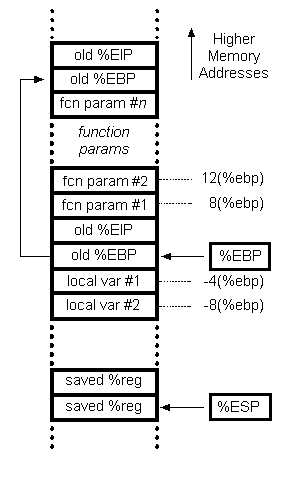
\includegraphics[width=0.5\textwidth]{imagenes/stack.png}
  \caption{Esquema que muestra de forma grafica la representación de un stack en el hilo de ejecución del procesador.}
  \label{Fig 1}
\end{figure}
\begin{figure}
  \centering
    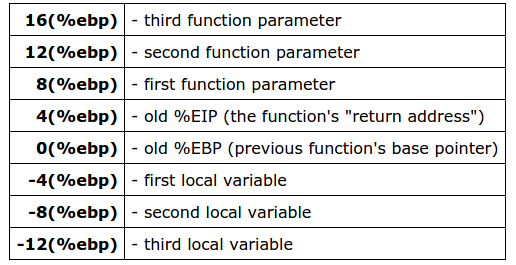
\includegraphics[width=0.5\textwidth]{imagenes/memory.png}
  \caption{Esquema que muestra la forma en la que esta compuesta un Stack Frame y sus punteros.}
  \label{Fig 2}
\end{figure}
La figura 3 muestra el flujo de funciones que utilizara la librería para determinar la traza de funciones. El diseño planteado propone que las funciones que deben ser escritas en Assembly son demarcadas con azul y las que deben ser escritas en C deben ser demarcadas con amarillo. La librería partirá por traceback que recibirá un puntero a un stack desde la función get\_ebp, luego esta función entrara en un bucle el cual se mantendrá hasta que no se reconozcan mas funciones desde la tabla después de haber encontrado la función main, obteniendo el siguiente Stack Frame a partir de la funcion get\_next\_ebp. En este bucle se buscara a través de la función search\_function, la cual obtiene el valor de retorno del Stack Frame a analizar y comienza a partir de las instrucciones previas, operación que se consigue restando 1 al puntero char que es asignado, a la dirección de retorno a buscar en un bucle a que función de la tabla corresponde. La labor de búsqueda se efectúa en la tabla con una función recursiva que recorre la tabla hasta encontrar coincidencia, en caso contrario se retornara y se pasara a analizar la siguiente instrucción. \\
Debido a que puede darse el caso en que jamas se encuentre una función en la tabla y por consecuente se genere un loop infinito, las búsquedas no podrán ser mas grandes que el tamaño máximo de una función. En caso de no encontrar ninguna coincidencia se retornara con un numero identificativo, que puede ser -1.
Existiendo un valor de posición valido de la tabla de funciones, se procede a analizar a través de la función print\_func, la cual imprimirá las funciones de acuerdo al formato solicitado.\\
Luego la función print\_func llamara a la función print\_args que hará uso de funciones programas en assembly para obtener los valores de los parámetros mencionados por la tabla de los cuales se verificara en caso de corresponder si es posible su impresión a través de la función isprint y isprint\_string.\\
Siguiendo este diagrama de desarrollo debería llegarse a una conclusión exitosa que responda a los requerimientos. Los detalles de construcción de las funciones están documentados por doxygen y el código escrito.

\begin{figure}
  \centering
    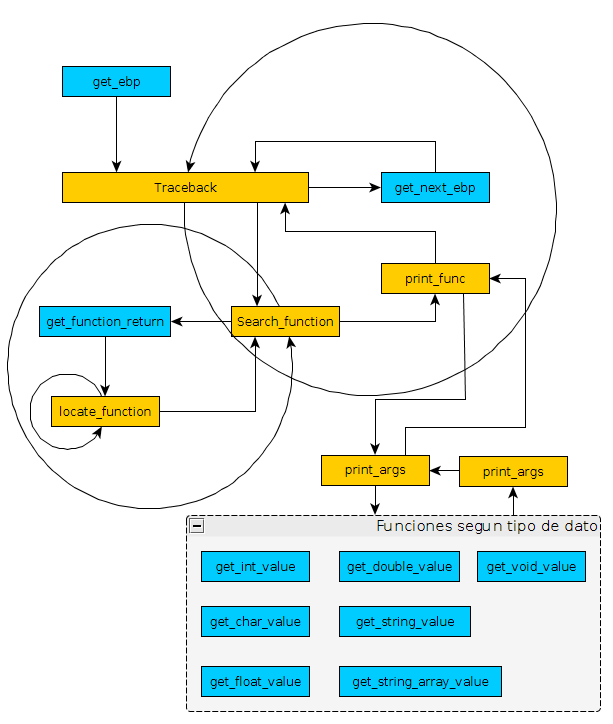
\includegraphics[width=0.5\textwidth]{imagenes/esquema.png}
  \caption{Esquema que muestra a modo explicativo el flujo de funciones que usa la librería traceback.}
  \label{Fig 3}
\end{figure}


\section{Desarrollo de la solución}
Siguiendo el diagrama de construcción planteado previamente propuesto, el desarrollo se concluyo con algunas incidencias que fueron corregidas e iteradas durante la codificación. Por ejemplo el compilador gcc no acepto el casting explicito de punteros, arrojando errores que fueron buscados en foros especializados con el objeto de buscar una solución sin éxito, luego de esto se decidió crear una función por cada tipo de argumento en Assembly. \\
Otra incidencia ocurría a la hora de cortar los String con tamaño superior a 25, al efectuar el corte en los 25 caracteres y agregar los puntos suspensivos ocurría que la variable char* agregaba 2 caracteres no imprimirles. los cuales podían ser reemplazados por caracteres si se quería. Como el tamaño máximo del string debiera ser 28 que corresponde a los 25 caracteres y los 3 puntos, se busco métodos los locación de memoria para el char* mediante el método malloc y alloc, con los mismo resultados, por lo que se descubrió que el problema ocurría al agregar el ultimo punto suspensivo.
Finalmente se opto por utilizar un método de concatenación de la librería string.h para concatenar los 3 puntos luego de aplicar un substring a la cadena.\\
Otra de las incidencias ocurridas fue al extraer numero flotantes a través de Assembly, debido a que para esta clase de numero existen operaciones especiales y deben ser tratados de una forma distinta a los números convencionales.
\section{Pruebas propuestas}
Para probar que la librería efectúa el fin deseado se diseño un archivo modificado de los test estándar que venían con el paquete. Se efectuaron modificaciones a verify\_test.c con el objeto de extender sus pruebas tratando de probar todos los puntos.Es necesario mencionar que el único aspecto que no se probo porque no se puedo reproducir en testing, pero que si se encuentra implementado, es la capacidad de imprimir funciones que no se encuentran en la tabla de funciones proporcionada. Las demás funcionalidades fueron puestas a pruebas con el objeto de cumplir con lo pedido. El archivo verify\_test modificado se encuentra junto con la librería entregada.
\section{Resultados esperados de la prueba}
Por un análisis del código de prueba y según las especificaciones del documento de requerimientos se debería obtener en pantalla una serie de Strings que indiquen que la librería genera los resultados esperados. La coincidencia indica que efectivamente se cumple con lo esperado de la librería. Para la el archivo modificado verify\_test.c se debería obtener el siguiente resultado:
\\
\\
function f8(int i=5, char** f={"foo", "bar", Dirección de memoria, ...}), in\\
function f7(int p=6, int g=7, int j=8, int l=8), in\\
function f6(char* gato="abcdefghijklmnopqrstuvwxy..."), in\\
function f5(double array=4529999999999999...)in\\
function f4(int i=5, float f=35.000000), in\\
function f3(int p=6, char g=f, char l='\textbackslash6'), in\\
function f2(void), in\\
function f1(char** array={"foo", "bar", "baz", ...}), in\\
function main(void), in\\
.\\
.\\
.\\
function (wrapper)
\\\\
Luego de esto el programa no encontrara mas Stack Frame por lo que termina su ejecución con un FATAL, indicando que no existen mas funciones en el stack de llamada de la función traceback.
\section{Resultados Obtenidos}
Después de depurar el código eliminando todos las alertas de warning, lo cual genero un código limpio en C. la ejecución de verify\_test arrojo los siguientes resultados que se indican en la figura 1. La ejecución de la prueba 	se realizo en un equipo con linux, distribución Ubuntu 14.04.
\\
\begin{figure}
  \centering
    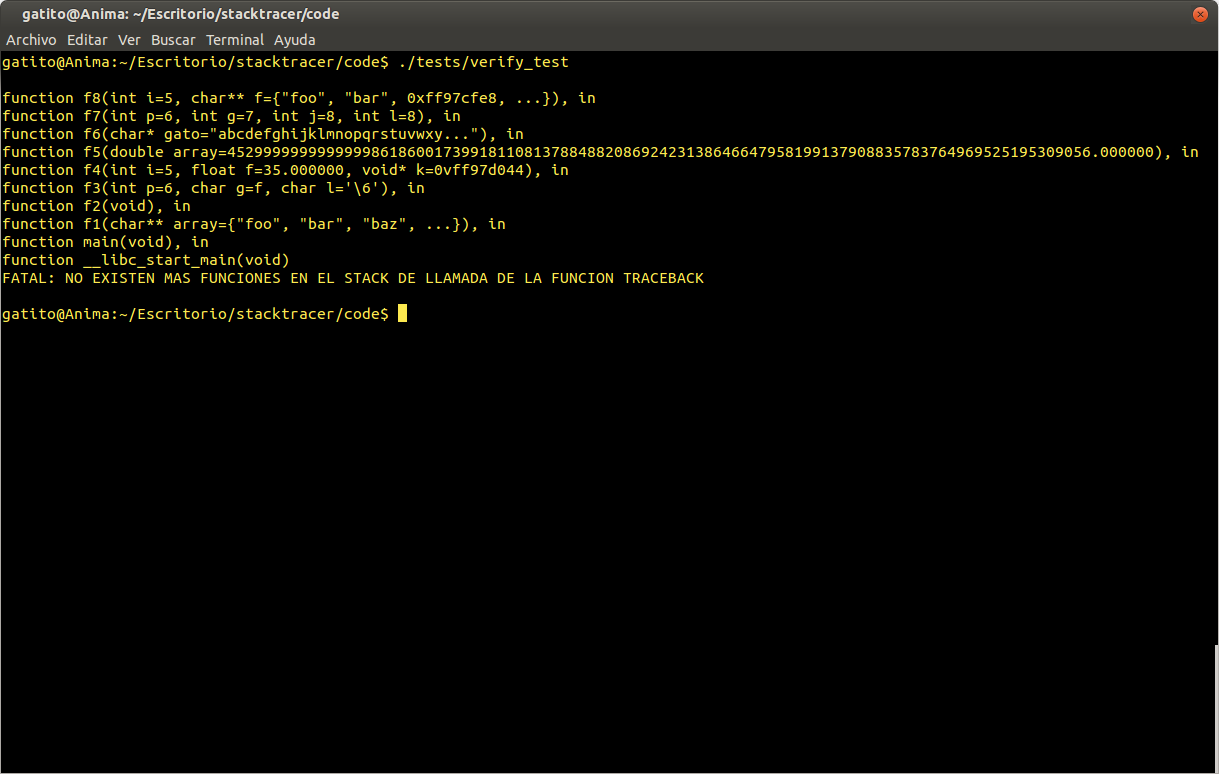
\includegraphics[width=0.5\textwidth]{imagenes/test.png}
  \caption{Imagen muestra los resultados obtenidos para el archivo de pruebas verify\_test, se observa que los resultados obtenidos concuerdan con los resultados esperados.}
  \label{Fig 4}
\end{figure}
La figura 4 muestra que los resultados obtenidos concuerdan con lo esperado por la ejecución de la librería. Se observa que la primera función mostrada es la que llamo a la librería traceback que corresponde a f8 y los parámetros indicados son los que se utilizaron en el código, flujo que posteriormente va mostrando uno a uno los resultados. \\
Los parámetros son impresos de forma correcta de acuerdo a las convenciones indicadas por los requerimientos y se sigue el flujo natural del programa hasta la función wrapper que es la encargada de llamar a main, que viene a ser la primera después de main. Luego de eso nos encontramos con que no existen mas funciones reconocibles en el Stack y la ejecución del programa termina con un FATAL.
Este es el comportamiento esperado para la librería, por lo que por relaciona lógica, la librería cumple con lo solicitado y esta lista para ser integrada por otro proyecto.
\section{Conclusiones}
Del presente trabajo practico y el desarrollo de la librería traceback se pueden concluir los siguientes puntos:\\
\begin{enumerate}
\item El lenguaje de programación C es altamente eficiente a la hora de construir librerías que actúen a bajo nivel, pero en ciertos casos es necesario interfaces en Assembly x86 para efectuar operaciones que C de forma nativa no es capaz de ejecutar.
\item EL lenguaje de programación Assembly Intel x86 provee poderosas herramientas para efectuar operaciones a nivel de hardware, pero por sus limitados registros de uso general se hace necesario el uso de un lenguaje de alto nivel como C para generar de una forma mas rápida y amigable operaciones complejas. Si bien es posible realizar todo con lenguaje Assembly por un tema de comodidad es mejor efectuar una mezcla entre código Assembly x86 y C, aunque se corre el riesgo que debido a las operaciones de optimización del copilador de C se efectúen simplificaciones que el programador no tiene contempladas.
\item Los registros \%EBP, \%ESP y \%EIP son punteros importantes a la hora de manipular Stack Frames ya que nos permiten acceder a los espacios de memoria asignados a las funciones los cuales operan a partir del puntero \%EBP. Las operaciones de desplazamiento de bytes que se pueden efectuar en estos punteros nos permiten, obtener los parámetros de cada función, así como los puntos en que fueron llamadas. Esto gracias a la tabla suministrada nos permite detectar la traza de funciones que se genera.
\item Los registros de coma flotante como float y double y long double, poseen operaciones especiales en Assembly x86, por lo que al utilizar esta clase de valores, es necesario utilizar los comandos para coma flotante siguiendo la sintaxis de sufijos para las asignaciones de memoria.
\item La librería traceback tiene interesantes aplicaciones en el campo de los debuggers, ya que podríamos hacer la traza de funciones que ocurren cuando se arroja una excepción de error. Características similares ocurren en el núcleo de JAVA al ocurrir errores y se le llama stacktrace.
\end{enumerate}
\section{Bibliografia}
\begin{enumerate}
\item Friedl's,Steve; Intel x86 Function-call Conventions - Assembly View; http://unixwiz.net/techtips/win32-callconv-asm.html
\item University of Virginia Computer Science; x86 Assembly Guide; http://www.cs.virginia.edu/~evans/cs216/guides/x86.html
\item Using Assembly Language in Linux; http://asm.sourceforge.net/articles/linasm.html
\item Intel Corporation; Intel® 64 and IA-32 Architectures
Software Developer’s Manual; http://home.ifi.uio.no/griff/INF5063/IA32Doc/Intel-IA32-Arch-SW-Dev-Man-Vol2A.pdf
\end{enumerate}
\end{document}